\documentclass{article}
\usepackage{color}
\usepackage{graphicx}
\usepackage{amsmath}
\usepackage[margin=0.75in]{geometry}

\begin{document}
\let\thefootnote\relax\footnotetext{Last edited March 14, 2015 by KO}


\section{Data preprocessing}
We split the data by year, 1990 and 2010, in which the sodium data was recorded.  We removed Chile from the analysis because there was no life expectancy data for 2010. 36 countries remained.  \\

There was no data on alcohol consumption in Taiwan.  We imputed the missing 2010 sex-specific alcohol consumption for Taiwan using a linear regression of male and female life expectancy, male and female salt consumption, and per capita GDP on sex-specific alcohol consumption in 2010 for all countries. Then we imputed the missing 1990 overall alcohol consumption for Taiwan in the same way, regressing predictors on overall alcohol consumption in 1990 for all countries. \\
 
There was no data for overall alcohol consumption levels in 2010, so we imputed them. A country's population average alcohol consumption was estimated by taking a weighted average of the country's male and female alcohol consumption, weighting by the proportion of males and females in the population.  On the other hand, there was no sex-specific alcohol consumption data for 1990.  For each country, we used the proportion of alcohol consumption in 2010 attributable to males and females to estimate the male and female sex-specific alcohol consumption in 1990, respectively, using the formula

$$\text{Male ETOH in 1990} \approx \text{Overall ETOH in 1990} \times \frac{\text{ Male ETOH in 2010}}{\text{ Imputed overall ETOH in 2010}}$$

\noindent A similar formula applies to females. \\

Finally, we took the difference between 2010 and 1990 for all (numeric) variables and split the data by sex.

\section{Sodium consumption and life expectancy}

We tested the hypothesis of association between sodium intake and excess mortality.  In our dataset, ``excess mortality'' is signified by a decrease in life expectancy from 1990 to 2010 beyond what would be expected given the other characteristics of a country.  We measured this by modeling the change in life expectancy using alcohol consumption and per capita GDP.  For our dataset, we fit several predictive models (ordinary linear regression, linear regression with polynomial terms, regression trees, bagged regression trees, random forests, boosted trees, and neural networks).  For each type of model, we tuned the parameters by training on bootstrap samples of the data and choosing the tuning parameter that results in the smallest average prediction error.  Finally, we among these tuned models, we chose the model with the smallest mean squared error.  For males, the model with best fit was a support vector machine with radial basis function kernel, and for females, the model with best fit was a random forest.  The residuals from these model represent the change in life expectancy not explained by alcohol consumption and per capita GDP. \\

We measured the strength of the association between sodium intake and the residuals from the model using Pearson's correlation. We tested the significance of the association using a permutation test.  Under the null hypothesis of no association, the residuals of the model are exchangeable: if sodium intake has no effect on mortality, then the residuals are equally likely to be paired with any of the sodium measurements.  Under the alternative hypothesis, our model will tend to \textit{overestimate} the increase in life expectancy from 1990 to 2010 in countries where sodium intake increased and to \textit{underestimate} the change in life expectancy in countries where sodium intake decreased. This alternative corresponds to a significant positive correlation between the residuals and change in sodium intake.  The correlation for males was $-0.0933$ (one-sided p-value $0.698$, two-sided p-value $0.594$) and the correlation for females was $-0.3302$ (one-sided p-value $0.9768$, two-sided p-value $0.0489$) (Figure~\ref{fig:sodium_excessmortality}). We conclude there is insufficient evidence to reject the null hypothesis that the correlation is $0$.  In fact, the correlation between change in sodium consumption and excess mortality for females is significantly less than $0$.  This means that for females in a particular country, an increase in sodium consumption is associated with a greater change in life expectancy than we would predict given that country's female alcohol consumption and per capita GDP. \\



\begin{figure}
\centering
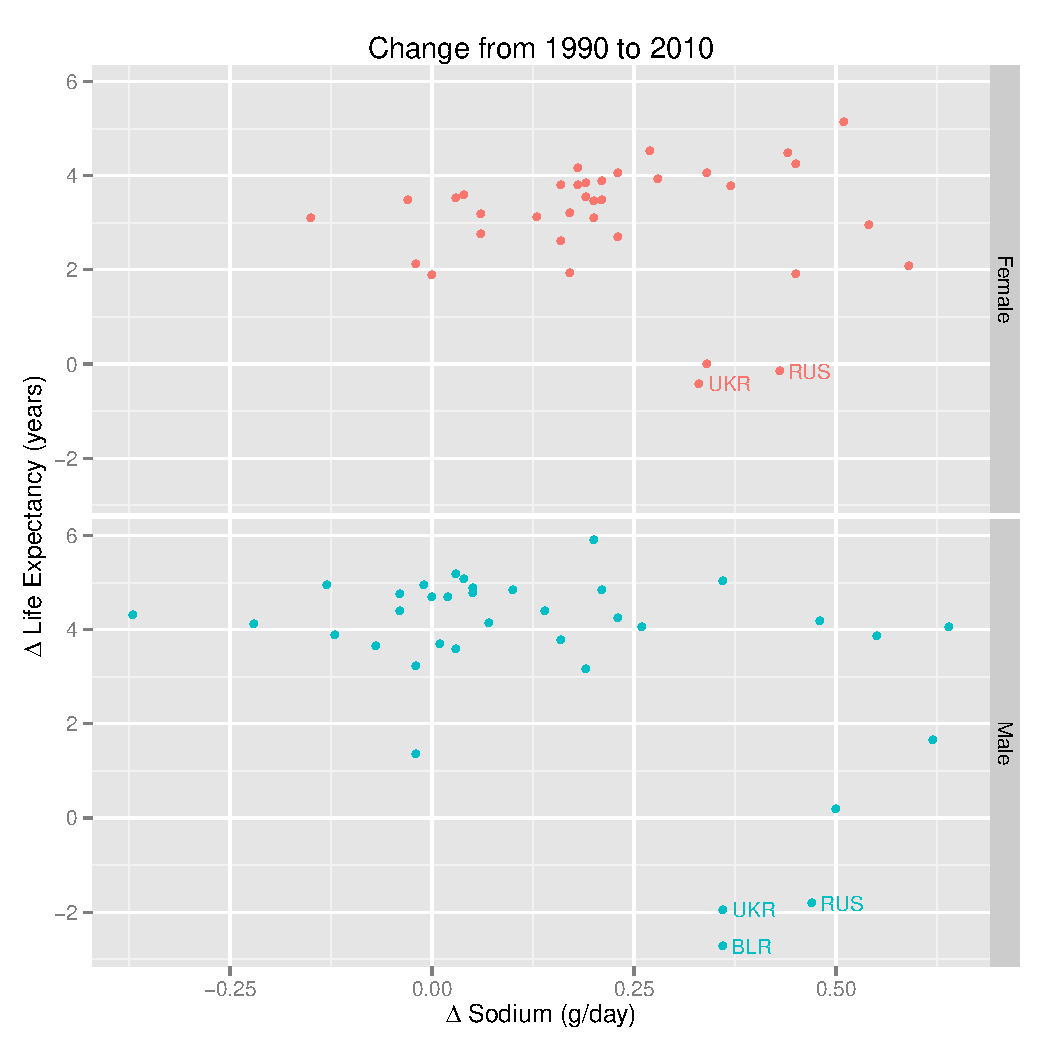
\includegraphics[scale = 0.75]{sodium_lifeexp.pdf}
\caption{Scatterplot of change in sodium intake against change in life expectancy at age 30 from 1990 to 2010. Even before correcting for the effect of other social and economic factors, there is no obvious association between sodium and life expectancy.}\label{fig:sodium_lifeexp}
\end{figure}

\begin{figure}
\centering
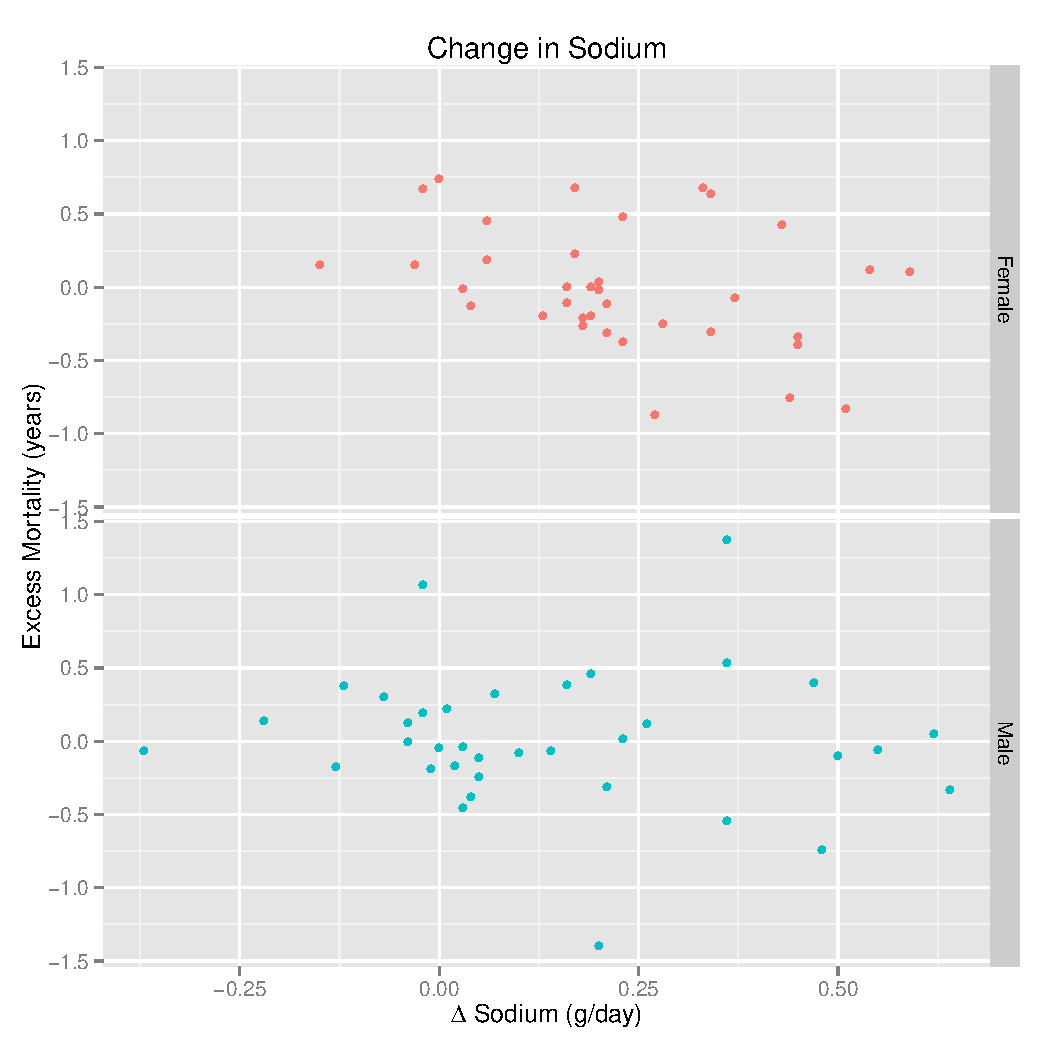
\includegraphics[scale = 0.75]{sodium_exmort.pdf}
\caption{Scatterplot of change in sodium intake against excess mortality.}\label{fig:sodium_excessmortality}
\end{figure}

\section{Smoking and life expectancy}
We repeated the analysis, switching the roles of sodium and cigarettes smoked.  Data preprocessing was identical to that of the first analysis, except...

\end{document}